\documentclass[11pt]{article}

\usepackage{fancyhdr}
\usepackage{tipa}
\usepackage{fontspec}
\usepackage{amsfonts}
\usepackage{enumitem}
\usepackage[margin=1in]{geometry}
\usepackage{graphicx}
\usepackage{float}
\usepackage{amsmath}
\usepackage{braket}
\usepackage{amssymb}
\usepackage{booktabs}
\usepackage{hyperref}
\usepackage{mathtools}
\usepackage{float}
\usepackage{algpseudocodex}
\usepackage{titlesec}
\usepackage{bbm}

\newcommand{\cnum}{ECE M146}
\newcommand{\ced}{Spring 2023}
\newcommand{\ctitle}[4]{\title{\vspace{-0.5in}\cnum, \ced\\Problem Set #1: #2}\author{\vspace{-0.35in}\\Name: #3, UID: #4}}
\newcommand{\solution}[1]{{{\color{blue}{\bf Solution:} {#1}}}}

\renewcommand*{\theenumi}{\alph{enumi}}
\renewcommand*\labelenumi{(\theenumi)}
\renewcommand*{\theenumii}{\roman{enumii}}
\renewcommand*\labelenumii{\theenumii.}

\newcommand{\R}{\mathbb{R}}
\newcommand{\norm}[1]{\left\lVert#1\right\rVert}

\DeclareMathOperator{\Cov}{Cov}
\DeclareMathOperator{\Var}{Var}
\DeclareMathOperator{\E}{E}
\DeclareMathOperator{\Tr}{Tr}
\DeclareMathOperator{\sign}{sign}



\begin{document}
\ctitle{0}{Environment Setup}{Kevin Sheng}{406 196 414}
\date{}
\maketitle

\section{Problem 1}

\solution{
      \begin{align*}
            \frac{\partial}{\partial x} x \sin(z) e^{-x}
             & = \sin(z) \left(e^{-x} + x \cdot -e^{-x}\right) \\
             & = \boxed{\sin(z) e^{-x} \left(1-x\right)}
      \end{align*}
}

\section{Problem 2}

\begin{enumerate}
      \item Problem 2a

            \solution{$y^Tz = 1 \cdot 2 + 3 \cdot 3 = \boxed{11}$}

      \item Problem 2b

            \solution{
                  \[Xy = \begin{pmatrix}
                              2 \cdot 1 + 4 \cdot 3 \\
                              1 \cdot 1 + 3 \cdot 3
                        \end{pmatrix}
                        = \boxed{\begin{pmatrix}
                                    14 \\ 10
                              \end{pmatrix}}\]
            }

      \item Problem 2c

            \solution{\[X^{-1}=\begin{pmatrix}
                              \frac{3}{2}  & -2 \\
                              -\frac{1}{2} & 1
                        \end{pmatrix}\]}

      \item Problem 2d

            \solution{$X$ is invertible, so it has rank $\boxed{2}$.}
\end{enumerate}

\pagebreak

\section{Problem 3}

\begin{enumerate}
      \item Problem 3a

            \solution{The mean is $\boxed{\frac{3}{5}}$}.

      \item Problem 3b

            \solution{\[\Var(X)=\E\left[X^2\right]-\mu^2=\frac{3}{5}-\frac{9}{25}=\boxed{\frac{6}{25}}\]}

      \item Problem 3c

            \solution{Assuming order matters, it's $\frac{1}{2^5}=\boxed{\frac{1}{32}}$}.

      \item Problem 3d

            \solution{Instinct (and Desmos) tells me the best is $\boxed{\frac{3}{5}}$}.

      \item Problem 3e

            \solution{\[P(X=T \mid Y=b) = \frac{0.1}{0.1+0.15}=\boxed{\frac{2}{5}}\]}
\end{enumerate}

\section{Problem 4}

\solution{
      The names for the formulas going down are:
      \begin{enumerate}[label=\roman*]
            \item Bernoulli
            \item Uniform
            \item Binomial
            \item Exponential
            \item Gaussian
      \end{enumerate}
}

\section{Problem 5}

\begin{enumerate}
      \item Problem 5a

            \solution{The mean is $p$ and the variance is $p(1-p)$.}

      \item Problem 5b

            \solution{$\Var(2X)=4\sigma^2$ while $\Var(X+2)=\sigma^2$}.
\end{enumerate}

\section{Problem 6}

\begin{enumerate}
      \item Problem 6a

            \solution{$f$ and $g$ are both constant multiples of each other, so $f=\Theta(g)$.}

      \item Problem 6b

            \solution{$g=O(f)$ but not vice versa.}

      \item Problem 6c

            \solution{$g=O(f)$ but not vice versa.}
\end{enumerate}

\section{Problem 7}

\solution{
      If $X$ and $Y$ are independent, then
      \begin{align*}
            \E[XY]
             & = \int_{\infty}^{\infty} x \cdot \int_{-\infty}^{\infty} yf(x, y)\,dy\,dx  \\
             & = \int_{\infty}^{\infty} x \cdot \int_{-\infty}^{\infty} yf(x)f(y)\,dy\,dx \\
             & = \int_{\infty}^{\infty} xf(x) \cdot \int_{-\infty}^{\infty} f(y)\,dy\,dx  \\
             & = \int_{\infty}^{\infty} xf(x)\,dx \cdot \int_{-\infty}^{\infty} f(y)\,dy  \\
             & = \E[X]\E[Y]\quad\square
      \end{align*}
}

\section{Problem 8}

\begin{enumerate}
      \item Problem 3a
            \begin{enumerate}
                  \item 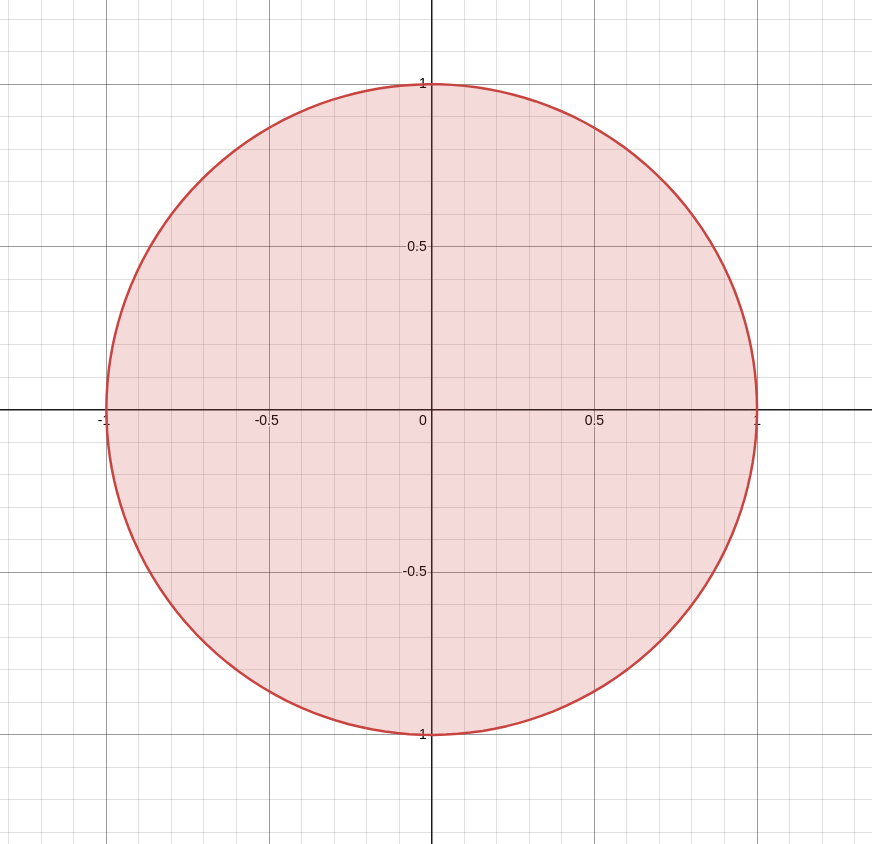
\includegraphics[width=7cm]{img/hw0/l2}
                  \item 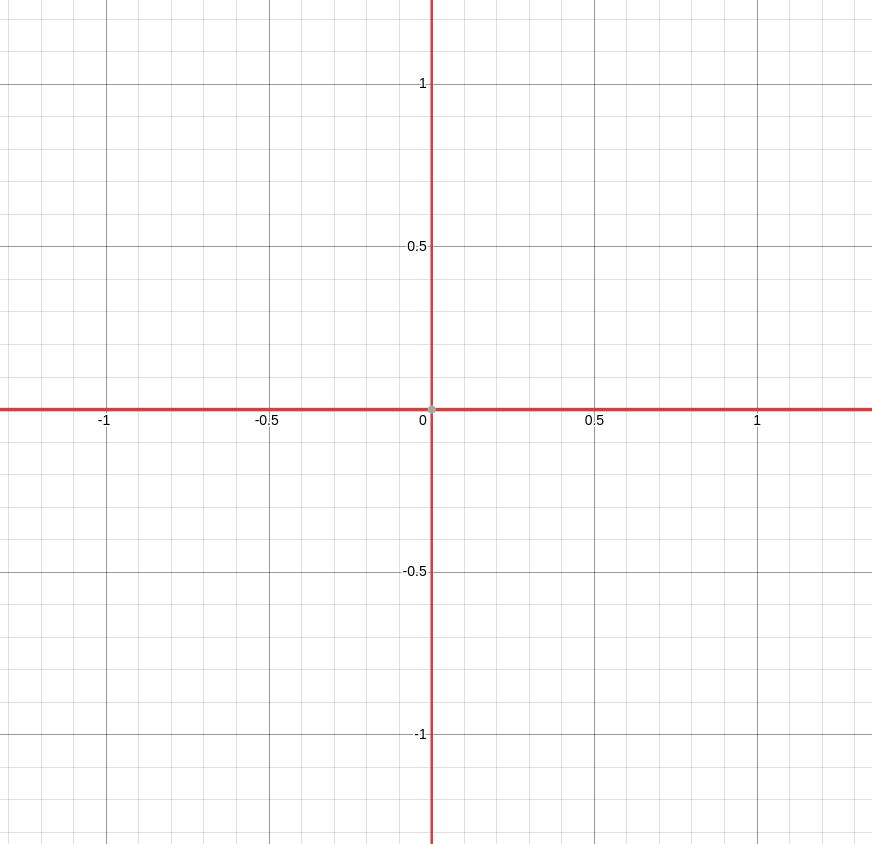
\includegraphics[width=7cm]{img/hw0/l0}
                  \item 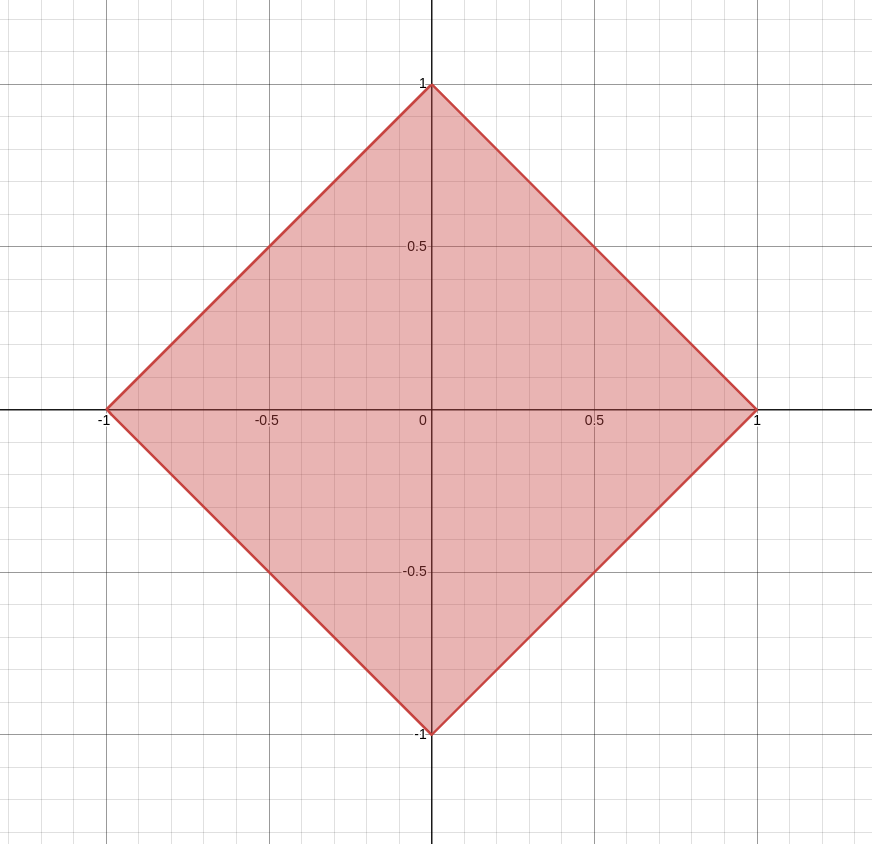
\includegraphics[width=7cm]{img/hw0/l1}
                  \item 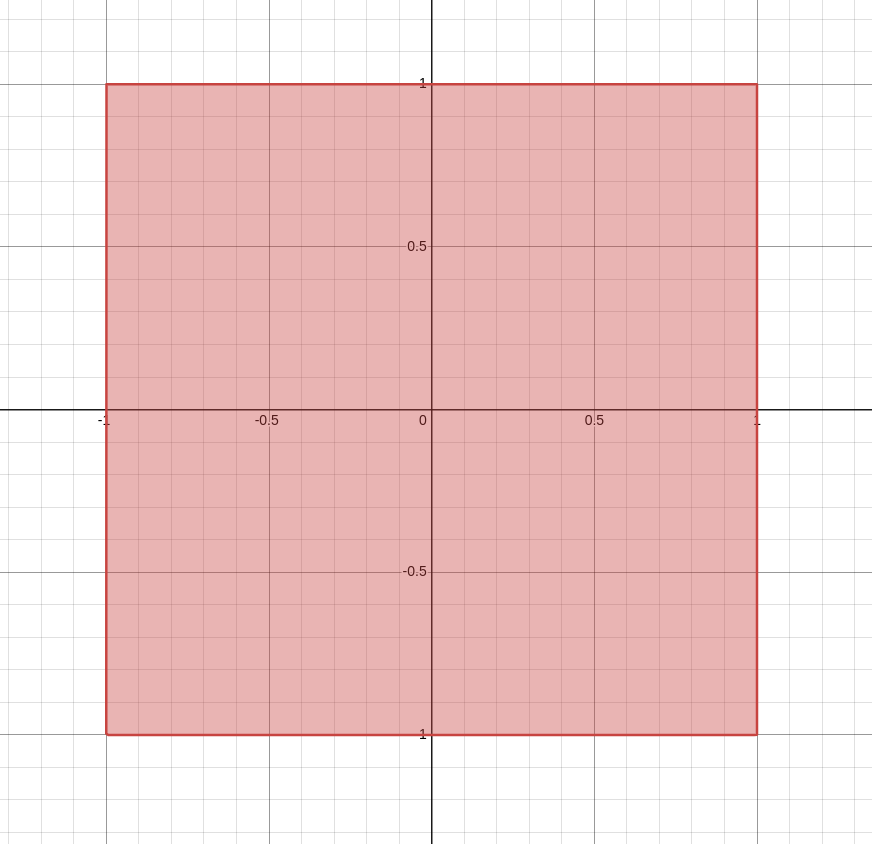
\includegraphics[width=7cm]{img/hw0/l_inf}
            \end{enumerate}

            \pagebreak

      \item Problem 3b

            \solution{\begin{enumerate}
                        \item A vector $v$ is called an eigenvector if $\exists c \in \mathbb{R}: Mv=cv$. \\
                              A scalar $c$ is called an eigenvalue if $\exists v: Mv=cv$.

                        \item Any eigenvalue $\lambda$ of $A$ must satisfy
                              \[\det(A-\lambda I)=(2-\lambda)^2-1=0\]
                              Solving this characteristic polynomial gets us $\boxed{\lambda \in \{1, 3\}}$.

                              For $\lambda=1$, the eigenvectors must satisfy
                              \[A\begin{pmatrix}
                                          x \\ y
                                    \end{pmatrix}=\begin{pmatrix}
                                          2x+y \\ 2y+x
                                    \end{pmatrix}=\begin{pmatrix}
                                          x \\ y
                                    \end{pmatrix}\]
                              so the vector must be in $\text{span}\left(\begin{pmatrix}
                                                1 \\ -1
                                          \end{pmatrix}\right)$.

                              As for $\lambda=3$, we have
                              \[\begin{pmatrix}
                                          2x+y \\ 2y+x
                                    \end{pmatrix}=\begin{pmatrix}
                                          3x \\ 3y
                                    \end{pmatrix}\]
                              so these vectors must be in $\text{span}\left(\begin{pmatrix}
                                                1 \\ 1
                                          \end{pmatrix}\right)$.

                        \item For any positive $k$ and eigenvector $v$, we have
                              \begin{align*}
                                    A^kv
                                     & = A^{k-1} \cdot Av        \\
                                     & = A^{k-1} \cdot \lambda v \\
                                     & = \lambda^k\quad\square
                              \end{align*}
                  \end{enumerate}}

      \item Problem 3c

            \solution{
                  \begin{enumerate}
                        \item $\frac{\partial}{\partial x} a^Tx=\boxed{a}$
                        \item $\frac{\partial}{\partial x} x^TAx=\boxed{\left(A^T+A\right)x}$, while the second derivative is just $\boxed{A^T+A}$.
                  \end{enumerate}
            }

      \item Problem 3d

            \solution{
                  \begin{enumerate}
                        \item Consider two points on the line $x_1$ and $x_2$:
                              \begin{align*}
                                               & w^Tx_1+b=w^Tx_2+b=0                                                  \\
                                    \implies{} & w^T(x_1-x_2)=0                                                       \\
                                    \implies{} & w \perp x_1-x_2\quad\square
                              \end{align*}
                        
                              \item The vector representing the shortest path to the line is probably orthogonal to it,
                              so it's probably some scalar multiple of $w$- call the closest point on the line $cw$.
                              
                              Thus, $w^T(cw)+b=0$, so $c=-\frac{b}{w^Tw}$
                              and the distance is $\frac{b||w||_2}{w^Tw}=\boxed{\frac{b}{||w||_2}}$.
                  \end{enumerate}
            }
\end{enumerate}

\pagebreak

\section{Problem 9}

\begin{enumerate}
      \item 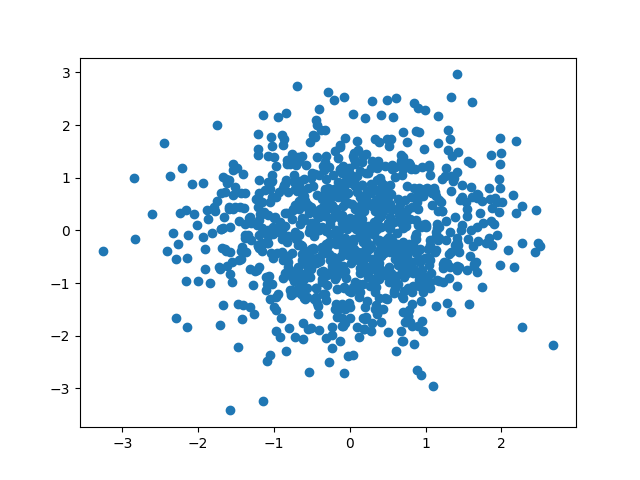
\includegraphics[width=7cm]{img/hw0/mpl_a}
      \item 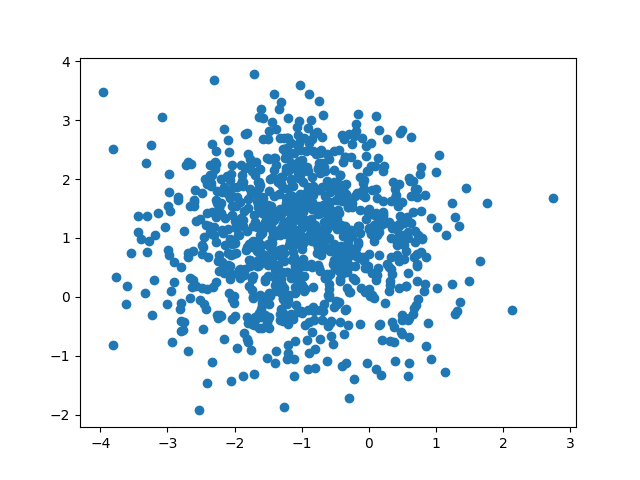
\includegraphics[width=7cm]{img/hw0/mpl_b}
      \item 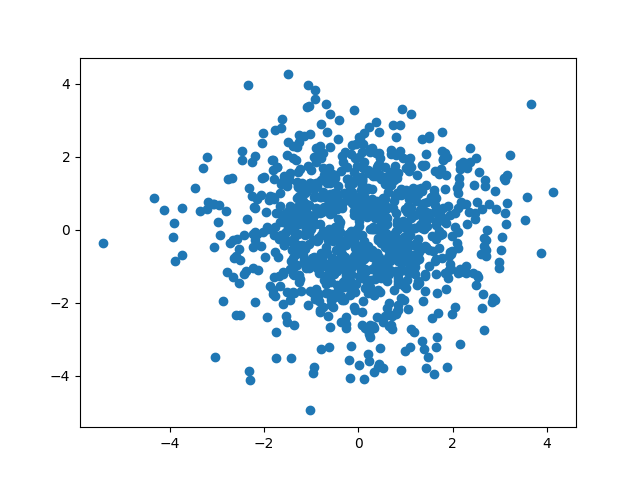
\includegraphics[width=7cm]{img/hw0/mpl_c}
      \item 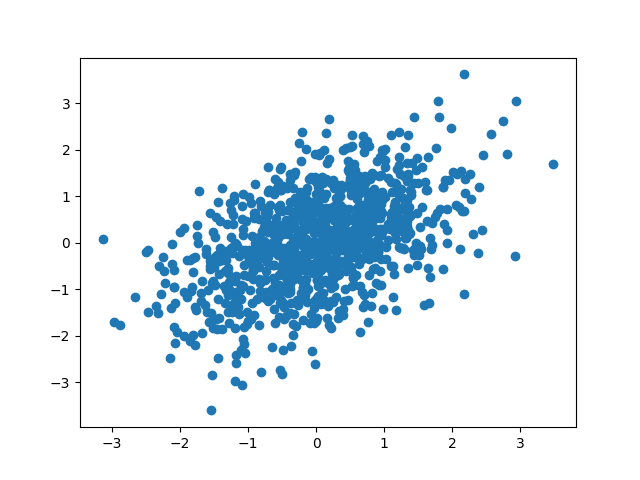
\includegraphics[width=7cm]{img/hw0/mpl_d}
      \item 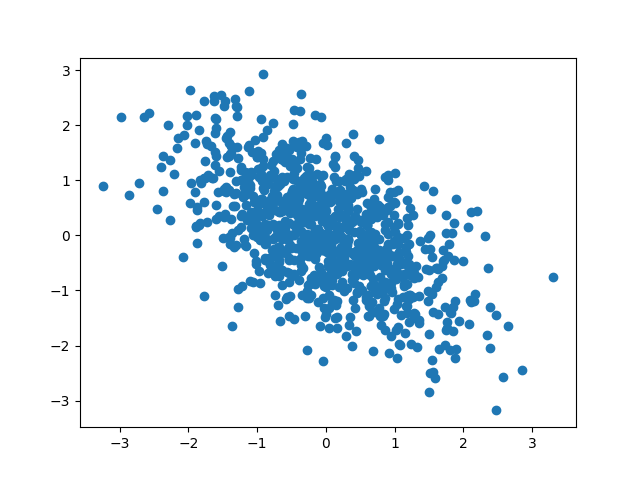
\includegraphics[width=7cm]{img/hw0/mpl_e}
\end{enumerate}

\section{Problem 10}

\solution{
      The larger eigenvalue is $\lambda=3$
      and the corresponding eigenvector is approx. $\begin{pmatrix}
            0 \\ 0.894
      \end{pmatrix}$
}

\section{Problem 11}

\solution{
      \begin{enumerate}
            \item The Iris dataset.
            \item It can be obtained {\color{red} \href{https://openml.org/search?type=data&status=active&id=61}{here}}.
            \item The dataset catalogues a bunch of iris flowers and their relevant measurements.
            \item There's only 150 instances.
            \item Each instance has 4 features.
      \end{enumerate}
}

\end{document}
